\chapter{Implementation}



\section{LSP server}

Our tool is integrated into IDEs via the Language server protocol. The goal is to give
users of the tool an overview of all clones as they appear in source-code.

The tool shows error-messages (diagnostics in LSP terms) which indicate which section of
code a clone covers, they also provide information about the matching clone and a
code-action to navigate to it.

The following user-stories shows how interaction with the LSP server works.

\begin{itemize}
	\item A programmer wants to see code clones for a file in their project, the
	      programmer opens the file in their IDE and is displayed diagnostics in the code
	      wherever there are detected clones. The matching code clones are not necessarily
	      in the same file.

	\item A programmer wants to see all code clones for the current project. The
	      programmer opens the IDEs diagnostic view and will see all code clones detected
	      as diagnostics there. The diagnostic will contain information like where the clone
	      exists, and where the matching clone(s) are.

	\item A programmer wants to jump to the corresponding match of a code clone in their
	      editor. The programmer moves their cursor to the diagnostic and will see a list of
	      the matching code clones. The programmer will select the wanted code clone which
	      will move the cursor to the file and location of the selected code clone.
          Alternatively, a code-action can be invoked to navigate, if the client does not
          implement the \verb|DiagnosticRelatedInformation| interface.

      \item A programmer wants to remove a set of clones by applying the
          ``extract-method'' refactoring. The programmer performs the necessary
          refactorings, saves the file and will get quick feedback whether the
          clones are now gone.
\end{itemize}

% TODO redo this figure
\begin{figure}
	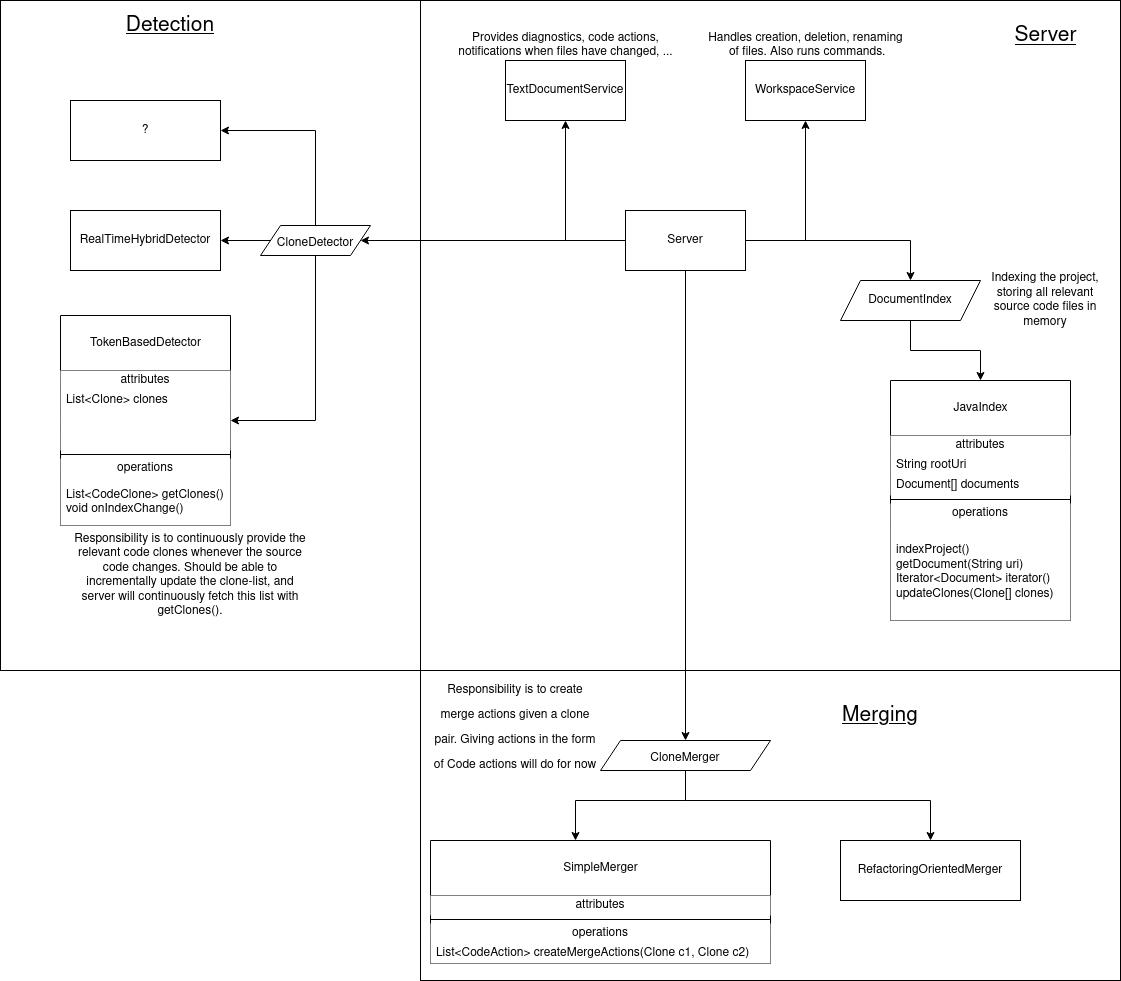
\includegraphics[width=\textwidth]{images/ToolArchitecture.png}
	\caption{Tool architecture}
	\label{fig:architecture}
\end{figure}

Figure \ref{fig:architecture} shows the architecture of the tool. The server communicates
with the IDE and delegates the work of managing clones to the detection engine and the
merge engine. The tool also stores an index of all source code files in the current project.

\subsection{Document index}

Upon starting, the LSP server requires indexing of the project for conducting analysis.
This involves creating an index and inserting the relevant documents. A document contains the
content of a file along with extra information such as the file's URI and information
about its clones.

There are two things to consider when determining which files should be inserted into the
index. First, we are considering only files of a specific file type, since the tool does
not allow analysis of multiple programming languages at the same time. Therefore, the
index should contain for example only \verb|*.java| files if Java is the language to
analyze. Secondly, all files of that file type might not be relevant to consider in the
analysis. This could for example be generated code, which likely contains a lot of
duplication, but is not practical or necessary to consider as duplicate code, since this
is not code which the programmer interact with directly. Therefore, the default behavior
is to consider only files of the correct file type, which are checked into Git. The tool
supports adding all files in a folder, or all files checked into Git.

When a document is first indexed by the server, the file contents is read from the disk.
However, as soon as the programmer opens this file in their IDE, the source of truth for
the files content is no longer on the disk, as the programmer is changing the file
continuously before writing to the disk. The LSP protocol defines multiple RPC
messages which the client sends to the server in order for the server to keep track of
which files are opened, and the state of the content of opened files.

Upon opening a file, the client will send a \verb|textDocument/didOpen| message to the
server, which contains the URI for the opened file. The index will at this point set the
flag \verb|isOpened| for the relevant document and stops reading its contents from disk.
Instead, updates to the file are obtained via the \verb|textDocument/didChange| message.
This message can provide either the entire content of the file each time the file changes,
or it can provide only the changes and the location of the change. Receiving only the
changes will be useful for this algorithm when the analysis incrementally reparses the
document.

\subsection{Displaying and interacting with clones}

\section{Clone detection algorithm}

\subsection{Fragment selection}

\subsection{Fingerprinting}

\subsection{Suffix array construction}

\subsection{Clone detection}

\subsection{Source-mapping}

\subsection{Incremental updates and optimizations}
